\documentclass[11pt,oneside]{book}
\usepackage{fancyhdr}
\usepackage[a4paper,top=2cm,bottom=3cm,left=2cm,right=2cm,marginparwidth=1.75cm]{geometry}
\usepackage[utf8]{inputenc}
\usepackage{pdfpages}
\usepackage{times}
\usepackage{pax}
\usepackage{hyperref}

\hypersetup{
    colorlinks,
    linktoc=all,
    linkcolor=red,
}
\setlength{\paperwidth}{21cm}   % A4
\setlength{\paperheight}{29.7cm}% A4
\special{papersize=21cm, 29.7cm}
\pdfpageheight\paperheight
\pdfpagewidth\paperwidth
\setlength\topmargin{-5mm} \setlength\oddsidemargin{-0cm}
\setlength\textheight{24.7cm} \setlength\textwidth{16cm}
\setlength\columnsep{0.6cm}  \newlength\titlebox \setlength\titlebox{2.00in}
\setlength\headheight{5pt}   \setlength\headsep{0pt}
\setlength\footskip{1.0cm}
\setlength\parindent{0pt}

\pagestyle{plain}
\pagenumbering{arabic}
\setcounter{page}{86}

\begin{document}
\renewcommand{\headrulewidth}{0pt}
\AddToShipoutPicture*{
  \setlength{\unitlength}{1mm}
  \footnotesize

        
  \put(0,14){\parbox[t]{\paperwidth}{\centering 
  							\emph{Proceedings of the Workshop on Combating Online Hostile Posts in Regional Languages during Emergency Situations}, pages 86 - 94 \\ 
	  						May 27, 2022 \textcopyright 
							2022 Association for Computational Linguistics}}
  
}
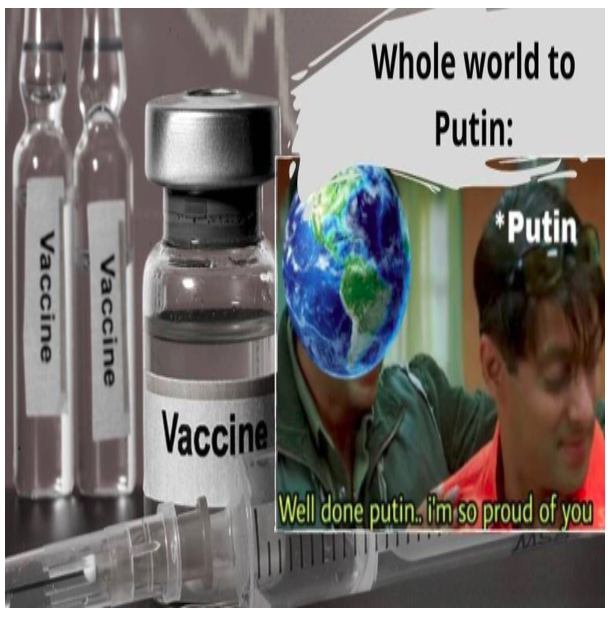
\includepdf[pagecommand={\thispagestyle{plain}},pages=-]{./papers/2.pdf}
\end{document}